
\begin{lead}
%\begin{nerai}
 本章では,ディジタル信号処理を学ぶ上で必要な数学的扱いの理解を行う.すなわち,解析に必要な三角関数,複素数,微分,積分,級数などを理解して,後で述べる内容が理解できるようにすることが目的である.

 高等学校における数学IIIや大学1~2年次における微分積分などが理解できているならば,この章を読み飛ばしても特に問題ないと思われる.

%\end{nerai}

%\vfill

%\begin{koumoku}
%微分\\
%積分\\
%複素数\\
%\end{koumoku}
\end{lead}

\chapter{数学的な基礎}
\label{chapter:2}

\clearpage

\section{複素数と三角関数}

ディジタル信号処理では,電気回路で多用される記号法による計算を知っていると役に立つことが多い.この記号法は,交流電気回路における電圧電流の関係が定常状態であるという条件のもと複素数を用いることで,微分方程式で表現される式から簡便に計算ができる特徴がある.このような計算を行うためには,複素数と三角関数との両方がよく理解されることが肝要である.

\subsection{複素数}\index{ふくそすう@複素数}

実数1と(実数体上)線形独立な$i$が$i^2 = -1$を満たすものとするとき,これを虚数単位という.ここで,$a$, $b$を実数として形式的に$a + bi$の形に書かれる式を一種の数と見なして複素数と呼ぶ.

任意の実数$a$は$a + 0i$と同一視して,実数の全体は自然に複素数の全体に埋め込むことができる(この埋め込みは,四則演算および絶対値を保つという意味で,位相体の埋め込みである).また任意の純虚数$bi$は$0 + bi$に同一視して複素数となる.

複素数$z = a + bi$に対して,
\begin{enumerate}
\item $a$を$z$の実部 (real part) といい,$\Re (z)$などで表す.
\item $b$を$z$の虚部 (imaginary part) といい,$\Im(z)$などで表す.ここで複素数の虚部は実数であって,虚数単位を含めた純虚数をいうのではないことに注意する.

\item 虚部が0でない,すなわち実数でない複素数のことを虚数という.
\item 実部が 0 である虚数は特に純虚数という.
\item 実部,虚部がともに整数のときガウス整数といい,その全体を$Z[i]$と書く.
\item 実部,虚部がともに有理数のときガウス有理数といい,その全体を$Q(i)$と表す.
\end{enumerate}

複素数$z = x + iy$と2つの実数$x$, $y$の組 $(x, y)$ は$1 : 1$に対応するから,複素数全体からなる集合$C$は,$z = x + iy$を$(x, y)$と見なすことにより,図\ref{fig:fukuso-heimen}に示すような座標平面と考えることができる.そこで$C$を複素数平面または単に数平面という.また,ガウス平面と呼ばれることもある.これと異なる語法として,$C$は複素数体上一次元のアフィン線形多様体であるので,複素直線とも呼ばれる.

数平面においては,$x$座標が実部,$y$座標が虚部に対応し,$x$軸(横軸)を実軸,$y$軸(縦軸)を虚軸と呼ぶ.

複素数$ z, w $に対して
\begin{equation}
d(z, w) = |z - w|
\end{equation}
とすると,$(C, d)$は距離空間となる.この距離は,座標平面におけるユークリッド距離に対応する.複素平面は複素数の形式的な計算を視覚化でき,数の概念そのものを拡張した.

\begin{figure}[H]
\begin{center}
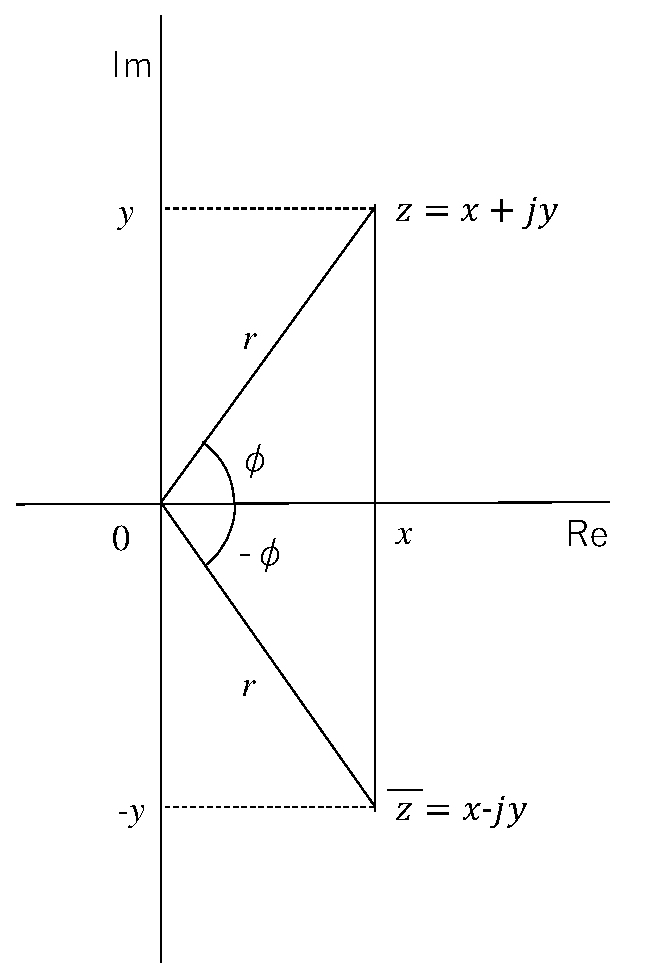
\includegraphics[width=.45\textwidth]{fig/zu-0-3-1.eps}
\end{center}
\caption{複素数と複素数平面}
\label{fig:fukuso-heimen}
\end{figure}

一般的に虚数単位は$i$で示されることが多いが,電気電子工学や情報工学の分野では,電流を表す変数として$i$を用いることから,これらを混同しないように虚数単位を$j$として表している.本書でも,その流れを汲んで虚数単位を$j$として表すこととする.

\subsection{極座標形式}

$x$軸および$y$軸をそれぞれ実軸および虚軸ととるのとは別の仕方で,複素数を複素数平面上の点$ P $として定義する方法として,原点$ O: (0,0) $からの距離と,正の実軸(英語版)と線分$ OP $の見込む角を反時計回りに測ったものの対($P$ の極座標)を考えることが挙げられる.これにより,複素数の\index{きょくざひょうけいしき@極座標形式}極座標形式の概念が導入される.

複素数$ z = x + yj $の絶対値とは
\begin{equation}
\displaystyle r=|z|={\sqrt {x^{2}+y^{2}}}
\end{equation}
で与えられる実数をいう.$z$が実数(つまり$ y = 0$)のとき$ r = |x| $は実数の絶対値$ (|x| = \max \{x, -x\}) $に一致する.一般の場合には,\index{ぴたごらすのていり@ピタゴラスの定理}ピタゴラスの定理により,$r $は原点と$ z $の表す点$ P $との距離に等しい.また,絶対値の平方は,自身とその\index{きょうやくふくそすう@共役複素数}共役複素数との積に等しい.すなわち複素数$ z $に対して
\begin{equation}
{\displaystyle |z|^{2}=z{\bar {z}}=x^{2}+y^{2}}
\end{equation}
が成り立つ.また,以下のような性質も成り立つ.

非退化性:$|z| = 0 ⇔ z = 0$

三角不等式:$ |z + w| \geqq |z| + |w| $

乗法性:$ |zw| = |z||w|$

\subsection{三角関数}\index{さんかくかんすう@三角関数}

\index{さんかくかんすう@三角関数}三角関数とは,平面三角法における,角の大きさと線分の長さの関係を記述する関数の族および,それらを拡張して得られる関数の総称である.鋭角を扱う場合,三角関数の値は対応する直角三角形の二辺の長さの比であり,三角関数は三角比とも呼ばれる.三角法に由来する三角関数という呼び名のほかに,後述する単位円を用いた定義に由来する円関数という呼び名がある.

三角関数には以下の6つがあり,図\ref{fig:sankakukansuu-tanien}にその関係を示す.
\begin{enumerate}
\item sin(正弦,sine)
\item sec(正割,secant)($\sec \theta = 1/\sin \theta$)
\item tan(正接,tangent)($\tan \theta = \sin \theta / \cos \theta$)
\item cos(余弦,cosine)
\item csc(余割,cosecant)($\csc \theta = 1/\cos \theta$)
\item cot(余接,cotangent)($\cot \theta = \cos \theta / \sin \theta$)
\end{enumerate}

\begin{figure}[H]
\begin{center}
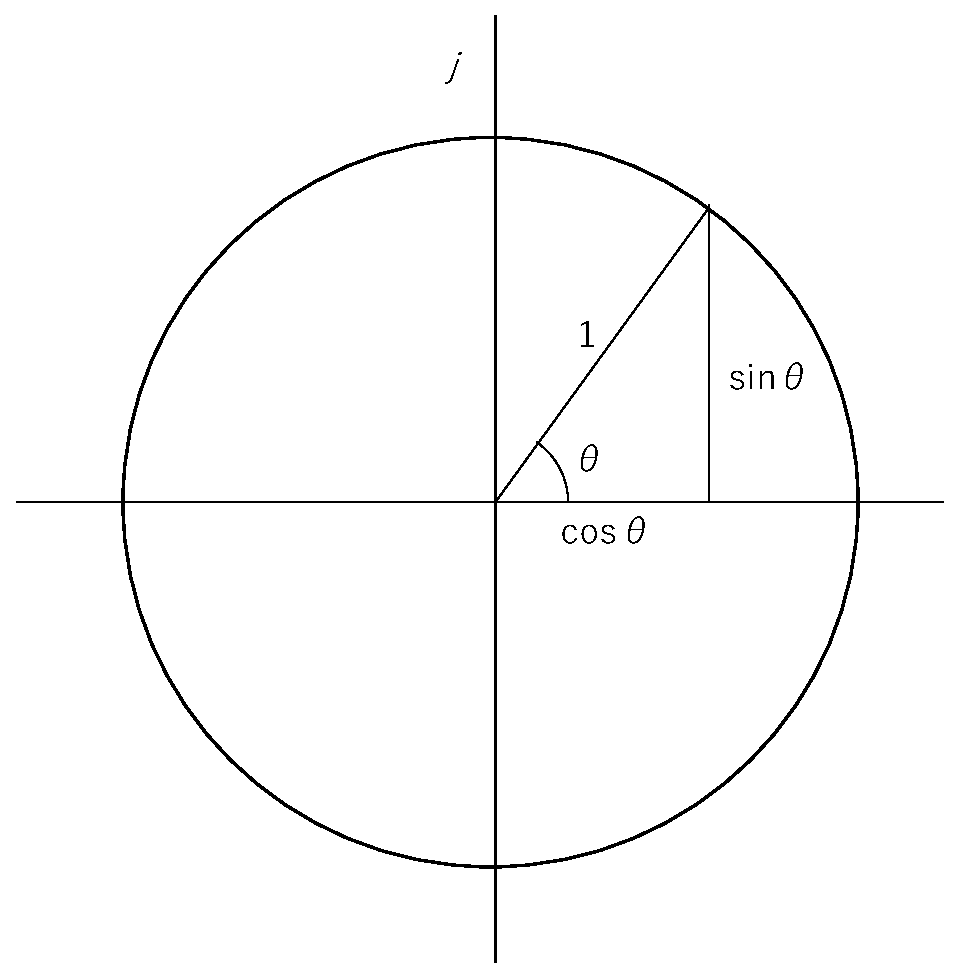
\includegraphics[width=70mm]{fig/zu-0-2-2.eps}
\end{center}
\caption{単位円を用いた三角関数の説明}
\label{fig:sankakukansuu-tanien}
\end{figure}

特に sin, cos は幾何学的にも解析学的にも良い性質を持っているので,さまざまな分野で用いられる.たとえば波や電気信号などは,正弦関数と余弦関数を組み合わせることで表現することができる.この事実はフーリエ級数およびフーリエ変換の理論として知られ,音声などの信号の合成や解析の手段として利用されている.他にもベクトルの外積や内積は正弦関数および余弦関数を用いて表すことができ,ベクトルを図形に対応づけることができる.初等的には,三角関数は実数を変数とする一変数関数として定義される.三角関数の変数の対応するものとしては,図形のなす角度や,物体の回転角,波や信号のような周期的なものに対する位相などが挙げられる.

三角関数に用いられる独特な記法として,三角関数の累乗と逆関数に関するものがある.
通常,関数$f(x)$の累乗は
$(f(x))^2=f(x) \cdot f(x)$
や
$(f(x))^{-1}=1/f(x)$
のように書くが,
三角関数の累乗は$\sin^2 x$のように書かれることが多い.
逆関数については通常の記法$(f^{-1}(x))$と同じく,
$\sin^{-1}x$
などと表す(この文脈ではしたがって,三角関数の逆数は分数を用いて 
$1/\sin x$
 のように,あるいは$(\sin x)^{-1}$ などと表される).文献あるいは著者によっては,通常の記法と三角関数に対する特殊な記法との混同を避けるため,三角関数の累乗を通常の関数と同様にすることがある.また,三角関数の逆関数として $-1$ と添え字する代わりに関数の頭に arc と付けることがある(たとえば sin の逆関数として$\sin^{-1}$の代わりに arcsin を用いる).

\subsection{オイラーの公式}

数学,特に複素解析における\index{おいらーのこうしき@オイラーの公式}オイラーの公式 (Euler's formula) は,指数関数と三角関数の間に成り立つ以下の関係をいう.
%\footnote{虚数単位$j$ \\
%虚数単位については$i^2=-1$となる2つの数のうちの1つの数のことをいう.そのような数のことを$i=\sqrt{-1}$として学習することが通例である.しかしながら,電気電子工学や情報工学などの分野では電流に関する変数を$i$と混同することを避けるために虚数単位として$j$を用いることが習慣となっている.}
\begin{equation}
{\displaystyle e^{j\theta }=\cos \theta +j\sin \theta .
}
\end{equation}
ここで $e^{\theta}$は指数関数,$j$は虚数単位,$\cos \theta$, $\sin \theta$はそれぞれ余弦関数および正弦関数である.任意の複素数$\theta$に対して成り立つ等式であるが,特に$\theta$が実数である場合が重要でありよく使われる.$\theta$が実数のとき,$\theta$は複素数 $e^{j\theta}$がなす複素平面上の偏角(角度$\theta$の単位はラジアン)に対応する.

オイラーの公式は,変数 $\theta$ が実数である場合には,右辺は実空間上で定義される通常の三角関数で表され,虚数の指数関数の実部と虚部がそれぞれ角度 $\theta$ に対応する余弦関数$\cos$と正弦関数$\sin$に等しいことを表す.このとき,偏角 $\theta$ をパラメータとする曲線$e^{j\theta}$ は,複素平面上の単位円をなす. 特に,$\theta = \pi$のとき(すなわち偏角が 180 度のとき),
\begin{equation}
{\displaystyle e^{j\pi }=-1}
\end{equation}
となる.この関係はオイラーの等式 (Euler's identity) と呼ばれる.



\section{極限}

\index{きょくげん@極限}
極限を求める式の一例として,
\begin{equation}
\lim_{x \rightarrow b}(x+a)=a+b
\end{equation}
と書く場合,ここでは$x$を$b$に限りなく近づけたら,$x+a$は$a+b$に限りなく近づく,という意味を持つ.

また,$\infty$とは限りなく大きいことを表す記号である.したがって,$\infty + \infty = 2\infty$と書くことはないので注意が必要である.
%
特に,$\infty - \infty$,$\infty \times 0$,$\infty / \infty$,$0/0$となる場合で極限を求めるときは,個々の問題によって工夫が必要であり,信号処理において是非知ってほしい式もこの極限を理解した上で利用することが求められる.

\subsection{$\infty - \infty$の場合}

例として,$\displaystyle \lim_{x \rightarrow \infty}(x^2-3x)$を求める.

\begin{eqnarray}
\lim_{x \rightarrow \infty}(x^2-3x) &=& \lim_{x \rightarrow \infty}x^2(1-\frac{3}{x}) \nonumber \\
&=& \infty
\end{eqnarray}

\noindent この場合は,最高次数の項$x^2$でくくり出すことで,極限が求められる.

もうひとつの例として,$\displaystyle \lim_{x \rightarrow \infty}(\sqrt{x^2+x}-x)$を求める.

\begin{eqnarray}
\lim_{x \rightarrow \infty}(\sqrt{x^2+x}-x) &=& \lim_{x \rightarrow \infty}\frac{(\sqrt{x^2+x}-x)(\sqrt{x^2+x}+x)}{\sqrt{x^2+x}+x} %\nonumber \\
 =  \lim_{x \rightarrow \infty}\frac{(x^2+x)-x^2}{\sqrt{x^2+x}+x} \nonumber \\
&=& \lim_{x \rightarrow \infty}\frac{x}{\sqrt{x^2+x}+x} %\nonumber \\
 =  \lim_{x \rightarrow \infty}\frac{1}{\sqrt{1+\frac{1}{x}}+1} %\nonumber \\
 =  \lim_{x \rightarrow \infty}\frac{1}{1+1} %\nonumber \\
 = \frac{1}{2}
\end{eqnarray}

\noindent この場合は,分母子に$\sqrt{x^2+x}+x$を掛けて分子を有理化し,分母子をともに最高次数の項$x$でくくり出すことで,有限値の極限が求められる.

\subsection{ロピタルの定理}

\index{ろぴたるのていり@ロピタルの定理}ロピタルの定理は以下のように表現される.

\begin{enumerate}
\item 関数$f(x)$,$g(x)$が$x=a$を含む区間$I$で連続である\footnotemark .
\item 区間$I$の$x \neq a$で微分可能かつ$g'(x) \neq 0$である.
\item $\displaystyle \lim_{x \rightarrow a} f(x) = \lim_{x \rightarrow a} g(x) = 0$または$\pm \infty$($0/0$または$\infty/\infty$の不定形)である.
\item $\displaystyle \lim_{x \rightarrow a} \frac{f'(x)}{g'(x)} = A$ $(-\infty \leq A \leq \infty)$が存在する.
\end{enumerate}

\footnotetext{この$f'(x)$,$g'(x)$は,それぞれ$f(x)$,$g(x)$の\index{どうかんすう@導関数}導関数といわれるものであり,詳細は\ref{subsection:doukansu}項を参照されたい.
}

上記1.~4.を満たすとき,$\displaystyle \lim_{x \rightarrow a} \frac{f(x)}{g(x)} =\displaystyle \lim_{x \rightarrow a} \frac{f'(x)}{g'(x)} = A$が成り立つ.

ここで$a$が$\pm \infty$や$a\pm 0$の場合であっても成り立つ.

さらに,4.を満たす限り,不定形が解消されるまで繰り返し適用することができる.

\subsection{$\infty / \infty$の場合}

例として,$n$を正の整数とした場合の$\displaystyle \lim_{x \rightarrow \infty}(x^n e^{-x})$を求める.
\begin{equation}
\lim_{x \rightarrow \infty}(x^n e^{-x}) = \lim_{x \rightarrow \infty}\frac{x^n}{e^{x}} %\nonumber \\
 =  \lim_{x \rightarrow \infty}\frac{nx^{n-1}}{e^{x}} =%\nonumber \\
    \cdots %\nonumber \\
 =  \lim_{x \rightarrow \infty}\frac{n!}{e^{x}} %\nonumber \\
 =  0
\end{equation}
この場合は,ロピタルの定理を用いることにより容易に求めることができる.

\subsection{$0 / 0$の場合}

例として,信号処理においては重要な関数であるsinc関数$\displaystyle (\frac{\sin x}{x})$について,$\displaystyle \lim_{x \rightarrow 0}\frac{\sin x}{x}$を求める.

\begin{eqnarray}
\lim_{x \rightarrow 0}\frac{\sin x}{x} &=& \lim_{x \rightarrow 0}\frac{\cos x}{1} \nonumber \\
&=& 1
\end{eqnarray}

\noindent この場合も,ロピタルの定理を用いれば容易に求めることができる.

\subsection{はさみうちの原理}

関数における``\index{はさみうちのげんり@はさみうちの原理}はさみうちの原理''は以下の通りである.

$f(x) \leq g(x) \leq h(x)$かつ$\displaystyle \lim_{x \rightarrow A}f(x)=\lim_{x \rightarrow A}h(x)=\alpha$なら$\displaystyle \lim_{x \rightarrow A}g(x)=\alpha$となる.

以上のようなはさみうちの原理も,極限を求める際に有効な方法のひとつである.

適用例として,信号処理においては重要な関数であるsinc関数$\displaystyle(\frac{\sin x}{x})$について,$\displaystyle \lim_{x \rightarrow \infty}\frac{\sin x}{x}$を求める.

この$\displaystyle\frac{\sin x}{x}$の分子に着目すると,$\displaystyle -1 \leq \sin x \leq 1$である.この性質を利用すると,$x>0$であるときに,
\begin{equation}
\displaystyle \frac{-1}{x} \leq \frac{\sin x}{x} \leq \frac{1}{x}
\label{eqn:eqn-hasami-uchi}
\end{equation}
となり,この不等式の$\displaystyle \frac{-1}{x}$ならびに$\displaystyle \frac{1}{x}$は$x$を無限に大きくすると,ともに0となることから,その間にある$\displaystyle \frac{\sin x}{x}$も0になるため,
\begin{equation}
\displaystyle \lim_{x \rightarrow \infty}\frac{\sin x}{x}=0
\end{equation}
となる.

このようにはさみうちの原理を利用することによって極限が求められた\footnote{ここでは$x \rightarrow \infty$の場合であれ,$x \rightarrow -\infty$の場合であれ,分子の値が有限の値を持つことから,$\displaystyle\frac{\sin x}{x}$は$0/0$や$\infty / \infty$のような不定形はとらないので,ロピタルの定理は適用できない.}.


\section{微分}

一般的に「\index{びぶん@微分}微分するとは,導関数を求めること」と高校生のとき以降より習ってきていることであろうが,このことを説明するために,
\begin{enumerate}
\item 平均変化率
\item 微分係数
\item 導関数
\item 微分する
\end{enumerate}
の順に説明する.

\newpage
\subsection{平均変化率}

図\ref{fig:zu-0-01}に示すように,変数$x$が$a$から$b$まで変化するとき,関数$y=f(x)$の\index{へいきんへんかりつ@平均変化率}平均変化率$\Delta y/\Delta x$は
%\footnote{式(\ref{eqn:eqn-0-1})の分子}{この式の分子は,
%\begin{eqnarray}
%& &(y-f(b))-(y-f(a)) \nonumber \\
%&=&f(b)-f(a) \nonumber
%\end{eqnarray}
%となる.
%}
\begin{equation}
\frac{\Delta y}{\Delta x}=\frac{yの増加量}{xの増加量}=\frac{f(b)-f(a)}{b-a}
\label{eqn:eqn-0-1}
\end{equation}

である.すなわち,2つの点A$(a,f(a))$,B$(b,f(b))$を通る直線の傾きを表すものを平均変化率という.

\begin{figure}[H]
\begin{center}
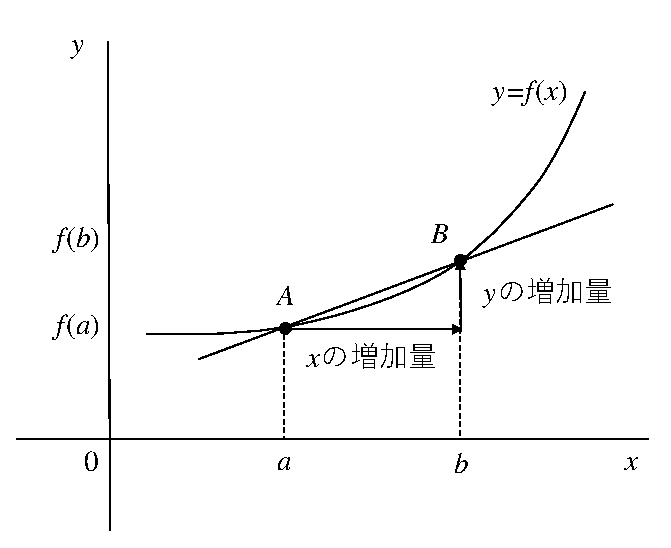
\includegraphics[width=80mm]{fig/zu-0-01.eps}
\end{center}
\caption{平均変化率}
\label{fig:zu-0-01}
\end{figure}

\subsection{微分係数}

先述の平均変化率において,$b$を限りなく$a$に近づけた値
\begin{equation}
f'(a)=\lim_{b \rightarrow a}\frac{f(b)-f(a)}{b-a}
\label{eqn:eqn-0-01}
\end{equation}
を\index{びぶんけいすう@微分係数}微分係数という.

図\ref{fig:zu-0-02}において,2つの点A$(a,f(a))$,B$(b,f(b))$を通る直線は,点Bを点Aに限りなく近づけたとき,点A$(a,f(a))$における接線に近づく.その結果,微分係数は関数$y=f(x)$のグラフにおける点A$(a,f(a))$における接線の傾きを表すということができる.

ここで$b$と$a$との差$h=b-a$とおくと,式(\ref{eqn:eqn-0-01})は
\begin{equation}
f'(a)=\lim_{h \rightarrow 0}\frac{f(a+h)-f(a)}{h}
\label{eqn:eqn-0-02}
\end{equation}
と書くことができる.

\begin{figure}[H]
\begin{center}
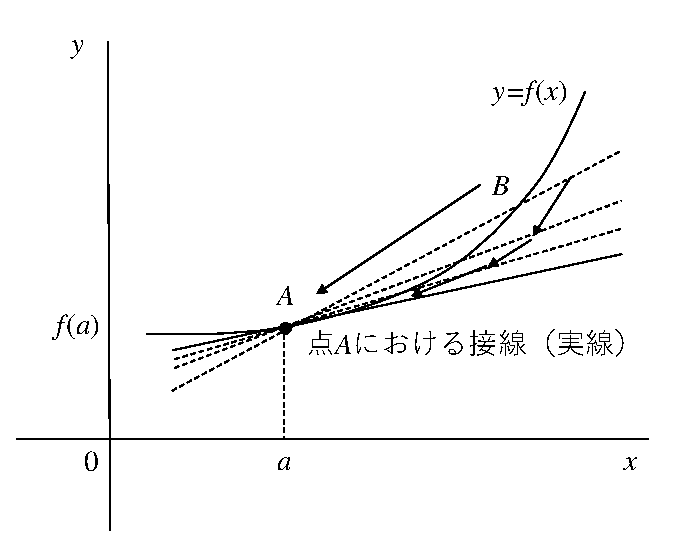
\includegraphics[width=80mm]{fig/zu-0-02.eps}
\end{center}
\caption{微分係数}
\label{fig:zu-0-02}
\end{figure}

\subsection{導関数}
\label{subsection:doukansu}

微分係数$f'(a)$を求めるための式(\ref{eqn:eqn-0-02})は,$a$を$x$軸上のどこにとるかによって値が決まるので$a$の関数すなわち導関数と呼ぶ.ここで,改めて$a$を$x$とおくことで導関数$f'(x)$は,
\begin{equation}
f'(x)=\lim_{h \rightarrow 0}\frac{f(x+h)-f(x)}{h}
\label{eqn:eqn-0-03}
\end{equation}
と書くことができる.このように,導関数とは微分係数が求められる関数のことをいう.
詳しい導出は省略するが,主として用いる導関数は表\ref{table:table0-1}に示される.

\begin{table}[H]
\caption{導関数の例}
\label{table:table0-1}
\begin{center}
\begin{tabular}{c|c}
\hline
関数$f(x)$ & 導関数$f'(x)$ \\
\hline
$x$ & 1 \\
\hline
$x^n$ & $nx^{n-1}$ \\
\hline
$e^x$ & $e^x$ \\
\hline
$\sin x$ & $\cos x$ \\
\hline
$\cos x$ & $-\sin x$ \\
\hline
$\log x$ & $\displaystyle \frac{1}{n}$ \\
\hline
$g(x)h(x)$ & $g'(x)h(x)+g(x)h'(x)$ \\
\hline
$f(g(x))$ & $f'(g(x))g'(x)$ \\
\hline
$\displaystyle \frac{1}{g(x)}$ & $\displaystyle \frac{g'(x)}{(g(x))^2}$ \\
\hline
\end{tabular}
\end{center}
\end{table}

\subsection{微分するとは}

微分するとは,導関数を求めることでもある.

ここで,図\ref{fig:zu-0-1}に示すような曲線の関数を
\begin{equation}
y=f(x)
\end{equation}
とすると,$f(x)$の導関数$f'(x)$は,
\begin{equation}
y'=\frac{dy}{dx}=f'(x)=\frac{df(x)}{dx}
\end{equation}
と表現される.

また,$x$として定数$a$を代入したときの$f'(a)$を微分係数と呼ぶ.

%微分するということにあたっては,導関数を求めるということでもあるため,わかりにくい言い回しであるかも知れない.

\begin{figure}[H]
\begin{center}
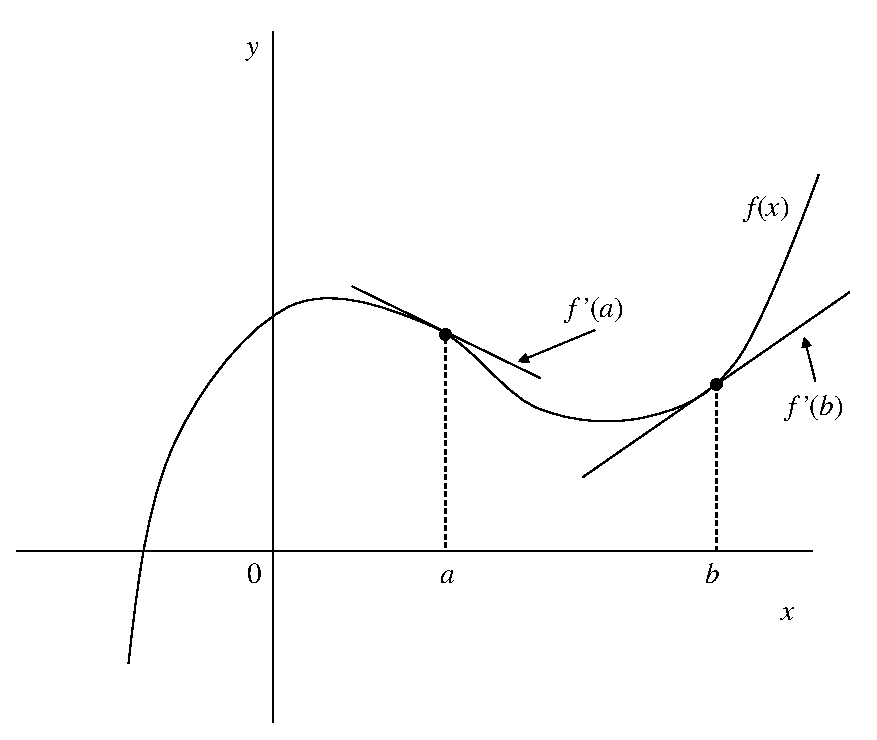
\includegraphics[width=.7\textwidth]{fig/zu-0-1.eps}
\end{center}
\caption{曲線とその傾き}
\label{fig:zu-0-1}
\end{figure}


\section{積分}

フーリエ変換や$z$変換などを習得する際に必要となってくるのは積分である.ここでは,積分について,
\begin{enumerate}
\item 不定積分と定積分とのちがい
\item 積分の計算方法
\end{enumerate}
について説明する.

\subsection{不定積分}

\index{ふていせきぶん@不定積分}不定積分とは,微分すると$f'(x)$になる関数$f(x)$のことである.すなわち,関数$f'(x)$の原始関数$f(x)$を求めることでもある.このことから関数と導関数との関係(たとえば表\ref{table:table0-1})がわかれば,不定積分を求めることができる.

たとえば,$x^2$の不定積分は
\begin{equation}
\int x dx = \frac{1}{2}x^2+C
\end{equation}
と書くことができる.ここで$C$は積分定数である.

\subsection{定積分}

定積分とは,$y=f(x)$と,$x=a$,$x=b$,$x$軸で囲まれた面積を求めることとして考えられる.ただし,$x$軸より下に存在する部分についてはマイナスの符号が付くものとして考える.

たとえば,$f(x)$の導関数を$f'(x)$とした場合であれば,
\begin{equation}
\int_{a}^{b}f'(x)dx = f(b)-f(a)
\end{equation}
と書くことができる.不定積分に見られる積分定数$C$は,この右辺で差がとられていることから存在しなくなる.

\subsection{不定積分と定積分とのちがい}

先述のことから,関数$f(x)$に対して,
\begin{itemize}
\item 不定積分とは,微分すると関数$f(x)$になる関数のこと
\item \index{ていせきぶん@定積分}定積分とは,不定積分に積分区間の両端の値を代入した値の差のこと
\end{itemize}
ということができる.

\subsection{積分の計算方法}

ここでは不定積分におけるいろいろな計算方法について説明する.

\subsubsection{関数の和}

2つの関数$f(x)$と$g(x)$との和に関する不定積分は,
\begin{equation}
\int(f(x)+g(x))dx = \int f(x)dx +\int g(x)dx
\end{equation}
として計算することができる.

\subsubsection{関数の積(\index{ぶぶんせきぶんほう@部分積分法}部分積分法)}

2つの関数$f(x)$と$g(x)$との積に関する不定積分は,
\begin{equation}
\int f(x)g(x) dx = F(x) g(x)+\int F(x)g'(x)dx
\end{equation}
として計算することができる.ただし,$F(x)$は$f(x)$の原始関数である.

例として,$\ln x$(底$e$とした$\log_{e}x$のことを$\ln x$と書く)の不定積分を求める.この場合は,$f(x)$を$1$,$g(x)$を$\ln x$として計算すればよいので,

\begin{eqnarray}
\int \ln x dx &=& x \ln x +\int x \cdot \frac{1}{x} dx \nonumber \\
 &=& x (\ln x +1) +C
\end{eqnarray}

\noindent となる.

\subsubsection{合成関数(\index{ちかんせきぶんほう@置換積分法}置換積分法)}

変数$x$について$x=g(t)$とおくと,$dx=g'(t)dt$の関係があるので,
\begin{equation}
\int f(x)dx = \int f(f(g(t))g'(t)dt
\end{equation}
として計算することができる.

例として,区間$(0<x<1)$における$1/(1+x^2)$の定積分を求める.ここで,
\begin{equation}
x=\tan\theta=\frac{\sin \theta}{\cos \theta}
\label{eqn:eqn-0-3-1}
\end{equation}
とおくと,
\begin{equation}
\frac{1}{1+x^2}=\frac{1}{1+\tan ^2 \theta}=\cos ^2 \theta
\end{equation}
と書くことができる.また,式(\ref{eqn:eqn-0-3-1})の両辺を微分すると
\begin{equation}
\frac{dx}{d\theta}=\frac{1}{\cos ^2 \theta}
\end{equation}
と書くことができる
\footnote{式(\ref{eqn:eqn-0-3-1})は$\displaystyle x=\frac{\sin \theta}{\cos \theta}$として$f(\theta)=\cos \theta$とすると,
$\displaystyle \frac{\sin \theta}{\cos \theta}=\frac{-f'(\theta)}{f(\theta)}$とおくことができる.このため,
$\displaystyle \frac{dx}{d\theta}=\frac{1}{(f(\theta))^2}=\frac{1}{\cos^2 \theta}$
と書くことができる.
}.ここで,区間$(0<x<1)$は区間$(0< \theta <\pi /4)$と置き換えられるので,
\begin{equation}
\int_{0}^{1} \frac{1}{1+x^2}dx= \int_{0}^{\pi /4} \cos^2 \theta \cdot \frac{1}{\cos^2 \theta} \cdot d\theta %\nonumber \\
 = \int_{0}^{\pi /4} d\theta %\nonumber \\
 = \frac{\pi}{4}
%\int_{0}^{1} \frac{1}{1+x^2}dx&=& \int_{0}^{\pi /4} \cos^2 \theta \cdot \frac{1}{\cos^2 \theta} \cdot d\theta \nonumber \\
% &=& \int_{0}^{\pi /4} d\theta \nonumber \\
% &=& \frac{\pi}{4}
\end{equation}
となる.



\section{数列と級数}

ディジタル信号処理を学ぶ上では級数を用いた計算が多く現れるので,級数のことを理解することで,解析を行いやすくなる.ここでは,\index{とうひきゅうすう@等比級数}等比級数や関数の\index{きゅうすうてんかい@級数展開}級数展開について説明する.

\subsection{等比数列}

まず,級数の例として,ディジタル信号処理のなかで多く出現する\index{とうひすうれつ@等比数列}等比数列を考える.信号そのものや$z$変換が無限和の形で表現される場合があり,\index{でんたつかんすう@伝達関数}伝達関数やハードウェア構成を簡略化するために必要なものである.さて,この等比数列は,初項を$a$として公比$r$とおけば,\\
 $a$, $ar$, $ar^2$, $ar^3$, $ar^4$ $\cdots$\\
と表されるものである.このような数列の和を
\begin{equation}
\sum_{k=1}^{n}r^{k} ar^{k-1}= a + ar + ar^2 + ar~3 + ar^4 + \cdots + ar^n
\end{equation}
と書く.ここで,

\begin{eqnarray}
(1-r)\sum_{k=1}^{n}r^{k-1} &=& (1-r)(1 + r + r^2 + r^3 + r^4 + \cdots + r^{n-1}) \nonumber \\
 &=& (1+r+r^2+ \cdots r^{n-1}) -r ((1+r+r^2+ \cdots r^{n-1})) \nonumber \\
 &=& 1-r^n
\end{eqnarray}

\noindent となることから,
\begin{equation}
\displaystyle \sum_{k=1}^{n} ar^{k-1}= \frac{a(1-r^n)}{1-r}
\end{equation}
と書くことができる.

$n \rightarrow \infty$の場合は無限等比級数の和ということだが,特に$|r|<1$の場合は
\begin{equation}
\displaystyle \sum_{k=1}^{\infty} ar^{k-1}= \frac{a}{1-r}
\end{equation}
と書くことができる.ただし,この無限等比級数の和が収束するのは$|r|<1$すなわち$-1 < r < 1$の場合だけである.


\subsection{関数の級数展開}

関数を,ある一点での導関数の値から計算される項の無限和として表すことができる.そのような級数を得ることをテーラー展開という.

一般的には,変数$x$の関数であるものとして,$x=a$のまわりでのテーラー展開は
\begin{equation}
f(x-a)=\displaystyle \sum_{n=0}^{\infty}\frac{f^{(n)}(a)}{n!}(x-a)^n
\end{equation}
と書くことができる.ここで$f^{(n)}(x)$は$f(x)$の$n$次導関数のことで,$n!$は$n$の階乗 ($n!=1\cdot 2 \cdot 3 \cdots n$) である.

たとえば,これを利用して,$e^x$について$x=0$のまわりでの\index{てーらーてんかい@テーラー展開}テーラー展開すなわち\index{まくろーりんてんかい@マクローリン展開}マクローリン展開は,

\begin{eqnarray}
e^x&=&1+x+\frac{x^2}{2!}+\frac{x^3}{3!}+\frac{x^4}{4!}+ \cdots \nonumber \\
&=& \sum_{n=0}^{\infty}\frac{x^n}{n!}
\end{eqnarray}\vskip.3\baselineskip

\noindent と$x$の多項式で表すことができる.

プログラミングの際,このような展開をすることによって多くの関数における数値計算が可能となっている.

\newpage

\section*{演習問題}

\subsection*{問題\ref{chapter:2}.1}

以下の複素数における絶対値と偏角を求めよ.
\begin{align}
(1) \hspace{3mm} & e^{-\pi/3} \nonumber & \qquad & &
(2) \hspace{3mm} &1+e^{-\pi/3} & \nonumber \\
(3) \hspace{3mm} & \displaystyle \frac{x+j3}{x-j3} \nonumber & \qquad & &
(4) \hspace{3mm} & \displaystyle R+j\omega L + \frac{1}{j\omega C} & \nonumber
\end{align}

\subsection*{問題\ref{chapter:2}.2}

(1) $0\leq \theta < 2\pi$のとき$\sqrt{3}\cos \theta -\sin \theta = 1$の$\theta$を求めよ.

(2) $\sin \theta + \cos \theta = \displaystyle \frac{2}{3}$のとき$\sin \theta \cos \theta$を求めよ.

\subsection*{問題\ref{chapter:2}.3}

以下の極限値を求めよ.
\begin{align}
(1) \hspace{3mm} & \lim_{x \rightarrow 1} \log_2 x \nonumber & \qquad & &
(2) \hspace{3mm} & \lim_{x \rightarrow 2} \displaystyle \frac{x^2-3x+2}{x^2-4} & \nonumber \\
(3) \hspace{3mm} & \lim_{x \rightarrow \infty } \displaystyle (\sqrt{x^2+3}-x) \nonumber & \qquad & &
(4) \hspace{3mm} & \displaystyle \lim_{x \rightarrow \infty} \displaystyle \frac{\sin x}{x} & \nonumber
\end{align}

\subsection*{問題\ref{chapter:2}.4}

次の関数を微分せよ.
\begin{align}
%(1) \hspace{3mm} y=(x+1)(x-1) \nonumber & \qquad &
(1) \hspace{3mm} & y=(x+1)(x-1) \nonumber & \qquad & &
%(2) \hspace{3mm} y=\displaystyle \frac{3x-1}{x^2-5} \nonumber \\
(2) \hspace{3mm} & y=\displaystyle \frac{3x-1}{x^2-5} & \nonumber \\
%(3) \hspace{3mm} y=\displaystyle \frac{x^2-1}{x^2+1} \nonumber & \qquad & 
(3) \hspace{3mm} & y=\displaystyle \frac{x^2-1}{x^2+1} \nonumber & \qquad & &
%(4) \hspace{3mm} y=\displaystyle \frac{1}{x\sqrt{x}} \nonumber \\
(4) \hspace{3mm} & y=\displaystyle \frac{1}{x\sqrt{x}} & \nonumber \\
%(5) \hspace{3mm} y=\sin (2-3x) \nonumber & \qquad &
(5) \hspace{3mm} & y=\sin (2-3x) \nonumber & \qquad & & 
%(6) \hspace{3mm} y=\tan (x-2) \nonumber \\
(6) \hspace{3mm} & y=\tan (x-2) & \nonumber \\
%(7) \hspace{3mm} y=e^{2x+5} \nonumber & \qquad &
(7) \hspace{3mm} & y=e^{2x+5} \nonumber & \qquad & & 
%(8) \hspace{3mm} y=e^{3x}\cos(2x+1) \nonumber \\
(8) \hspace{3mm} & y=e^{3x}\cos(2x+1) & \nonumber \\
%(9) \hspace{3mm} y=5^{x} \nonumber & \qquad &
(9) \hspace{3mm} & y=5^{x} \nonumber & \qquad & & 
\end{align}



\subsection*{問題\ref{chapter:2}.5}

以下の不定積分を求めよ.
\begin{align}
(1) \hspace{3mm} & \displaystyle \int (2x^3+3x^2-4x+5) dx \nonumber &  & &
(2) \hspace{3mm} & \int \displaystyle \frac{2}{\sqrt[3]{2x+3}} dx & \nonumber \\
(3) \hspace{3mm} & \int \{ 2\cos (4x+1) -\sin 2x \} dx \nonumber & & &
(4) \hspace{3mm} & \int \displaystyle \frac{e^{2x}+e^{-2x}}{e^x} dx & \nonumber \\
(5) \hspace{3mm} & \int \displaystyle \tan^2 2x dx & \nonumber & &
(6) \hspace{3mm} & \int \displaystyle e^{ax} \sin bx dx & \nonumber
\end{align}




\subsection*{問題\ref{chapter:2}.6}

以下の定積分の値を求めよ.
\begin{align}
(1) \hspace{3mm} & \displaystyle \int_{-1}^{3} (x^3-2x^2-3x+1) dx \nonumber &  & &
(2) \hspace{3mm} & \int_{1}^{4} \displaystyle \left ( \sqrt{x}+\frac{1}{x} \right ) dx & \nonumber \\
(3) \hspace{3mm} & \int_{0}^{\frac{\pi}{3}} ( 2\sin x -\cos 2x ) dx & & &
(4) \hspace{3mm} & \int_{-2}^{2} \displaystyle (e^x - e^{-x}) dx & \nonumber \\
(5) \hspace{3mm} & \int_{1}^{\sqrt{3}} \displaystyle \frac{dx}{\sqrt{4-3x^2}} & \nonumber & &
(6) \hspace{3mm} & \int_{0}^{1} \displaystyle \frac{dx}{3+x^2} & \nonumber
\end{align}


\subsection*{問題\ref{chapter:2}.7}

以下の無限級数について収束するようであればその和を求めよ.
\begin{align}
(1) \hspace{3mm} & 1+z^{-1}+z^{-2}+z^{-3}+\cdots & \nonumber  &  & 
(2) \hspace{3mm} & \displaystyle 1-\frac{1}{3}+\frac{1}{9}+\frac{1}{27}+\cdots & \nonumber 
\end{align}

\subsection*{問題\ref{chapter:2}.8}

以下の関数についてマクローリン展開せよ.
\begin{align}
(1) \hspace{3mm} & \cos x    \nonumber  &  
(2) \hspace{3mm} & \sin x   \nonumber &\\
(3) \hspace{3mm} & \log (1+x) \hspace{3mm}  (-1 < x \leq 1) &  & \nonumber 
\end{align}
